%!TEX root = ../../thesis.tex
\section{Introduction}
\label{sec: chap1 1_introduction}
Traditional robots are made from rigid and dense materials that ensure accurate and repeatable motions. While rigid robotics excel at fast and precise motion, their structural rigidity lacks the compliance and mechanical robustness needed for safe and passive interaction in an unknown environment. Soft robotics, on the other hand, aim to improve the motion complexity and environmental robustness that is generally lacking its rigid counterpart. To further promote these topics in robotics, researchers aim to mimic living creatures by developing bio-inspired robots with similar morphologies and mechanical properties \cite{Falkenhahn2015,Suzumori1991,Godage2015,Godage2016,Marchese2014,Kriegman2019}.
The hyper-flexible and continuum-bodied structure in soft robots provides them with a rich family of motion primitives. Besides bio-mimicry, soft robotics has proven to be a prominent alternative for rigid robotics with a variety of applications, \eg, manipulation and adaptive grasping \cite{Galloway2016}, untethered locomotion and exploration through uncertain environments \cite{Marchese2014,Choi2011,Pilz2020}, rehabilitation \cite{Polygerinos2015}, and even minimal-invasive surgery \cite{Li2017a,Cianchetti2014}. Although the popularity of the field has increased exponentially in recent years, one of the first soft robots dates back already to the early 1990s, \eg, the work of Suzumori et al. \cite{Suzumori1991}. Yet, despite years of soft robotics research, their intrinsic hyper-flexible nature still possesses numerous challenges on modeling and control.

One major challenge in modeling is that the soft robot's elastic body undergoes large, continuous deformation. Since its inception, numerous works have addressed the kinematics for soft continuum robots \cite{Jones2006,Mochiyama1999,Mochiyama2003}; yet, its original framework stems from hyper-redundant robotics nearly a decade earlier \cite{Chirikjian1994}. Similar to soft robots, hyper-redundant robots exploit their high joint redundancy to achieve a broader range of tasks (\eg, shape control and collision avoidance) besides end-effector manipulation. To some extent, soft robotics can be seen as the successor to hyper-redundant robotics in which rigid mechanical joints or links are substituted with hyper-flexible soft elements. \editl As such, the resulting dynamics involves one continuous deformable inertial body rather than a set of interconnected rigid bodies\editr. As such, conventional modeling approaches cannot be applied directly to these continuously deformable robots, stressing the importance of novel modeling strategies. In this respect, the dynamics of a continuously deformable soft robot are of infinite-dimensional nature. This paradigm shift has further emphasized the challenges in control-oriented modeling of soft robots, as their physical description are often more suited for a Partial-Differential Equations (PDEs) rather than Ordinary Differential Equations (ODEs).

Recently, some significant steps have been made toward formulating reduced-order ODE models for elastic continuum soft robots, paving a path toward model-based controllers. Perhaps one of the most popular techniques of spatial reduction is the so-called \textit{"Piece-wise Constant Curvature"} model -- PCC for short. The PCC model assumes that a soft robot's reachability can be described using a number of spatially-constant curves, which are parameterized using a minimal set of generalized coordinates. Although PCC models can be seen as a significant oversimplification of true continuum mechanics at hand, \editl and is only applicable within some conservative conditions on soft robots (\eg, elasticity dominates gravity)\editr, these models have proven to be remarkably viable for various control applications. Besides its use in inverse kinematic control \cite{Marchese2014,Marchese2016,Jones2006}, PCC models have also shown to be suitable for feedforward controllers as demonstrated by Falkenhahn et al. \cite{Falkenhahn2015}; and more recently, closed-loop feedback controllers by Della Santina et al. \cite{DellaSantina2020,Katzschmann2019}. Although the aforementioned works utilize the lumped-mass description, others have employed PCC models with uniform mass distribution \cite{Renda2018,Godage2015,Godage2016,Tatlicioglu2007,Tatlicioglu2007a} and current models even extend beyond the constant curvature \cite{Mochiyama2003,Chirikjian1994,DellaSantina2020}. However, in the face of significant external loading or (distributed) contact with the environment, the PCC assumption is relatively conservative and leads to undesired kinematic constraints on the continuum deformation. Besides, these models often need additional identification to model compliance as they do not originate from a continuum mechanical framework.

On the other hand, Finite-Element Method (FEM) models do originate from continuum mechanics and, due to their PDE description, provide a more accurate representation of deformations; and are particularly suited to deal with geometric and material nonlinearities. Duriez et al.\cite{Duriez2013} and related works \cite{Coevoet2017,Largilliere2015,Goury2018} showed that reduced-order FEM models could play an important role in closed-loop control -- allowing accurate volumetric deformation and hyper-elastic behavior. Although such real-time simulations for FEM-based models are possible, a significant state-reduction is required to ensure sufficient computational speed. In the process, FEM-based models often lose desirable control properties, \eg, passivity preservation, which might play an important role in control. An alternative modeling strategy is the recently emerging geometrically-exact Cosserat-beam model. Similar to the PCC models, the Cosserat models \editl benefit from their Lagrangian model structure \editr -- the basis for robotics control theory. Rooted in a geometric method for describing the continuum mechanics using Lie theory proposed by Simo et al. \cite{Simo1986}, Boyer et al. \cite{Boyer2010, Boyer2021} proposed a geometrically-exact modeling framework for Cosserat beams using nonlinear parametrization of the strain field. Other examples include the work of Renda et al. \cite{Renda2018,Renda2020}, providing various options for Piecewise-Constant Strain (PCS) and Variable Strain modeling approaches. Although recent variants of the Cosserat models offer good computational performance \cite{Till2019,Grazioso2019}, its use in model-based control is slowly upcoming.

In this respect, the topic of reduced-order modeling of soft robots is an active area of research. Yet, a challenge that is frequently overlooked in control-oriented research is the anisotropic material behavior, mechanical saturation, and more importantly, the nonlinear and possibly time-varying nature of the highly hyper-elastic soft materials \cite{Falkenhahn2015, Mochiyama2003, Till2019, Tatlicioglu2007}. This is further amplified by the fact that soft robots are known for their diversity in elastic materials and corresponding morphologies. Mustaza et al. \cite{Mustaza2019} proposed a modified nonlinear Kelvin-Voigt material model to embody the complex material behavior of silicone-composite manipulators (so-called STIFF-FLOP actuators). A similar silicone composite actuator was experimentally validated by Sadati et al.\cite{Sadati2020} who proposed a novel modeling approach with an appendage-dependent Hookean model and viscous power-law to describe nonlinear and time-dependent material effects, respectively. Both nonlinear material models show good correspondence with physical soft robots under various dynamic conditions, yet they lack general transferability to the soft robots with different geometries -- intrinsically captured by FEM-driven models. As of today, there are few control-oriented models that both offer geometry and material versatilely similar to FEM models and the control convenience similar to spatial curve models.

Ultimately, the strong nonlinearities paired with its continuous nature encourage the use of model-based controllers. Nevertheless, regarding the aforementioned model-based control approaches \cite{DellaSantina2020,Katzschmann2019,Falkenhahn2015}, the stability and performance of the closed-loop system could be undermined by uncertainties in physical parameters or unmodelled dynamics. Particularly for state-feedback linearization (e.g., inverse dynamic), as the inversion of inaccurately estimated systems could lead to poor performance and even instability. Adaptive control \cite{Slotine1988,Morgan1977} or energy-based controllers \cite{Ortega1998} might offer the needed robustness towards material uncertainties and unmodelled dynamics. Unfortunately, up till now, the applicability of adaptive and energy-based control techniques on soft robotics is scarcely explored. Franco et al. \cite{Franco2020} used an adaptive energy-based controller that compensates for external disturbances on the end-effector, yet this controller can be extended to include various slowly-varying material uncertainties, \eg, hyper-elasticity and viscosity.

%\pgfplotsset{colormap name = barney}
%\colormapcaption{0}{1cm}

The contributions here are two-fold. First, to derive a \editl finite-dimensional approximate of a soft continuum manipulator\editr, where we briefly recapitulate existing modeling techniques for soft robot manipulators. To address the issue of infinite-dimensionality, we explore the PCC condition that allows for a low-dimensional description of the continuum dynamics. Although such modeling approaches have been thoroughly developed, we will address two issues that will aid the development of model-based controllers. We aim to bridge the gap between the PCC model and the underlying continuum mechanics by matching the quasi-static behavior to a Finite-Element-driven model (FEM), and we propose a reduced-order integration scheme using Matrix-Differential Equations (MDEs) to compute the spatio-temporal dynamics in real-time. Preliminary results were shown in Caasenbrood et al. \cite{Caasenbrood2020,Caasenbrood2022}.
%

Second, in regards to the FEM-based hyper-elastic modeling and the possible presence of unmodelled dynamics (e.g., material uncertainties or external loads on the end-effector), a passivity-based adaptive controller is proposed that enhances robustness towards material uncertainties and unmodelled dynamics in closed-loop, slowly improving their estimates online.

\section{Pneumatic soft continuum manipulator}
By using additive manufacturing, we developed a soft and flexible robot manipulator that is suitable for pick-and-place applications. \editl The 3-DOF soft manipulator can be seen in Figure \ref{fig:C2:soft_robot} \editr.\editl The soft manipulators's design is reminiscent of the Orm robot developed by Scheinman \cite{BibEntryOrm2019Sep}, the composition of the network of soft actuators is loosely inspired by the elephant's trunk consisting mainly of parallel muscles without skeletal support\editr. The anatomy of the elephant's trunk provides an excellent study case, as it naturally exhibit continuum-body bending and moderate elongation \cite{Falkenhahn2015,Jones2006,Tatlicioglu2007}. \editl The design is also similar to other soft robotic systems \cite{Suzumori1991,Falkenhahn2015,Drotman2017} that all undergo three-dimensional movement by inflation or deflation of an embedded pneumatic bellow network\editr. The pneumatic network has three independent inputs, which are labeled $\uB = (u_1,\,u_2,\,u_3)^\top$. By varying these input, the \editl soft manipulator\editr can achieve bending in any preferred direction by differential pressurization of each channel ($<$0.1 \si{\mega \pascal}), \eg, $u_1 > u_2 = u_3 > 0$. Whereas, simultaneous pressurization accomplishes moderate elongation, \ie, $u_1 = u_2 = u_3$. As a demonstration, we provided the following pressure inputs to the system:
%
\begin{align}
  u_i(t) = \begin{cases}
          \;\;\erf(t)\cdot \left[P_0 - P_a\sin\left(\pi t + \delta\right)\right] \quad\;\; \textrm{for}\;\; i = 1,2 \\[0.35em]
          \;\;\erf(t)\cdot \left[P_0 - P_a\sin\left(\pi t \right)\right] \quad\quad\quad\;\; \textrm{for}\;\; i = 3\;\ \\
           \end{cases}
\end{align}
%
where $P_0 = 5$ \si{\kilo \pascal}, $P_a = 25$ \si{\kilo \pascal}, $\delta = \frac{\pi}{2}$, and $\textrm{erf}(t) := \frac{2}{\pi}\int_0^\tau \exp(-\tau^2) \; d\tau$   the error function to ensure a smooth transient. The demonstration is shown in Figure \ref{fig:C2:soft_robot}.

\begin{rmk}[Additive manufacturing] The soft \editl manipulator\editr is exclusively composed of a printable, flexible thermoplastic elastomer (Young's modulus $\le$ 80 \si{\mega \pascal}), which intrinsically promotes softness and dexterity. The elastomer material is developed explicitly for Selective Laser Sintering (SLS), a 3-Dimensional (3D) printing method that uses a laser to solidify powdered material. The main advantage of SLS printing over other techniques is that the printed parts are fully self-supported, which allows for highly complex and high-detail structures. It should be mentioned, though, that the layer-by-layer material deposition will introduce undesired anisotropic mechanical effects. To mitigate anisotropy, the bellows are printed orthogonal to the printing plane, thereby ensuring mechanical symmetry. For the majority of this work, the 3D-printed soft robot in Figure \ref{fig:C2:soft_robot} will form the basis of the dynamical model. The 3D model is made \editl publicly available at the  \sorotoki software repository found at \textnormal{\url{github.com/BJCaasenbrood/SorotokiCode}} \cite{Caasenbrood2020}. \editr
\end{rmk}

\begin{figure}[!h]
  \centering
  % This file was created by matlab2tikz.
%
%The latest updates can be retrieved from
%  http://www.mathworks.com/matlabcentral/fileexchange/22022-matlab2tikz-matlab2tikz
%where you can also make suggestions and rate matlab2tikz.
%
\begin{tikzpicture}

\begin{axis}[%
width=0.208\textwidth,
height=0.223\textwidth,
at={(0\textwidth,0.239\textwidth)},
scale only axis,
axis on top,
xmin=0.5,
xmax=1001.5,
tick align=outside,
y dir=reverse,
ymin=0.5,
ymax=1071.5,
axis line style={draw=none},
ticks=none
]
\addplot [forget plot] graphics [xmin=0.5, xmax=1001.5, ymin=0.5, ymax=1071.5] {./fig/fig_C2_srm_exampleV2-1.png};
\node[right, align=left, font=\color{white}]
at (axis cs:30,950) {\scriptsize $t = 0$ s};
\end{axis}

\begin{axis}[%
width=0.208\textwidth,
height=0.223\textwidth,
at={(0.247\textwidth,0.239\textwidth)},
scale only axis,
axis on top,
xmin=0.5,
xmax=1001.5,
tick align=outside,
y dir=reverse,
ymin=0.5,
ymax=1071.5,
axis line style={draw=none},
ticks=none
]
\addplot [forget plot] graphics [xmin=0.5, xmax=1001.5, ymin=0.5, ymax=1071.5] {./fig/fig_C2_srm_exampleV2-2.png};
\node[right, align=left, font=\color{white}]
at (axis cs:30,950) {\scriptsize $t = 1.3$ s};
\end{axis}

\begin{axis}[%
width=0.208\textwidth,
height=0.223\textwidth,
at={(0.494\textwidth,0.239\textwidth)},
scale only axis,
axis on top,
xmin=0.5,
xmax=1001.5,
tick align=outside,
y dir=reverse,
ymin=0.5,
ymax=1071.5,
axis line style={draw=none},
ticks=none
]
\addplot [forget plot] graphics [xmin=0.5, xmax=1001.5, ymin=0.5, ymax=1071.5] {./fig/fig_C2_srm_exampleV2-3.png};
\node[right, align=left, font=\color{white}]
at (axis cs:30,950) {\scriptsize $t = 2.6$ s};
\end{axis}

\begin{axis}[%
width=0.208\textwidth,
height=0.223\textwidth,
at={(0.742\textwidth,0.239\textwidth)},
scale only axis,
axis on top,
xmin=0.5,
xmax=1001.5,
tick align=outside,
y dir=reverse,
ymin=0.5,
ymax=1071.5,
axis line style={draw=none},
ticks=none
]
\addplot [forget plot] graphics [xmin=0.5, xmax=1001.5, ymin=0.5, ymax=1071.5] {./fig/fig_C2_srm_exampleV2-4.png};
\node[right, align=left, font=\color{white}]
at (axis cs:30,950) {\scriptsize $t = 3.9$ s};
\end{axis}

\begin{axis}[%
width=0.208\textwidth,
height=0.223\textwidth,
at={(0\textwidth,0\textwidth)},
scale only axis,
axis on top,
xmin=0.5,
xmax=1001.5,
tick align=outside,
y dir=reverse,
ymin=0.5,
ymax=1071.5,
axis line style={draw=none},
ticks=none
]
\addplot [forget plot] graphics [xmin=0.5, xmax=1001.5, ymin=0.5, ymax=1071.5] {./fig/fig_C2_srm_exampleV2-5.png};
\node[right, align=left, font=\color{white}]
at (axis cs:30,950) {\scriptsize $t = 5.1$ s};
\end{axis}

\begin{axis}[%
width=0.208\textwidth,
height=0.223\textwidth,
at={(0.247\textwidth,0\textwidth)},
scale only axis,
axis on top,
xmin=0.5,
xmax=1001.5,
tick align=outside,
y dir=reverse,
ymin=0.5,
ymax=1071.5,
axis line style={draw=none},
ticks=none
]
\addplot [forget plot] graphics [xmin=0.5, xmax=1001.5, ymin=0.5, ymax=1071.5] {./fig/fig_C2_srm_exampleV2-6.png};
\node[right, align=left, font=\color{white}]
at (axis cs:30,950) {\scriptsize $t = 6.4$ s};
\end{axis}

\begin{axis}[%
width=0.208\textwidth,
height=0.223\textwidth,
at={(0.494\textwidth,0\textwidth)},
scale only axis,
axis on top,
xmin=0.5,
xmax=1001.5,
tick align=outside,
y dir=reverse,
ymin=0.5,
ymax=1071.5,
axis line style={draw=none},
ticks=none
]
\addplot [forget plot] graphics [xmin=0.5, xmax=1001.5, ymin=0.5, ymax=1071.5] {./fig/fig_C2_srm_exampleV2-7.png};
\node[right, align=left, font=\color{white}]
at (axis cs:30,950) {\scriptsize $t = 7.7$ s};
\end{axis}

\begin{axis}[%
width=0.208\textwidth,
height=0.223\textwidth,
at={(0.742\textwidth,0\textwidth)},
scale only axis,
axis on top,
xmin=0.5,
xmax=1001.5,
tick align=outside,
y dir=reverse,
ymin=0.5,
ymax=1071.5,
axis line style={draw=none},
ticks=none
]
\addplot [forget plot] graphics [xmin=0.5, xmax=1001.5, ymin=0.5, ymax=1071.5] {./fig/fig_C2_srm_exampleV2-8.png};
\node[right, align=left, font=\color{white}]
at (axis cs:30,950) {\scriptsize $t = 9$ s};
\end{axis}

\begin{axis}[%
width=0.969\textwidth,
height=0.483\textwidth,
at={(-0.01\textwidth,-0.01\textwidth)},
scale only axis,
xmin=0,
xmax=1,
ymin=0,
ymax=1,
axis line style={draw=none},
ticks=none,
axis x line*=bottom,
axis y line*=left
]
\end{axis}
\end{tikzpicture}% \\[0.5em]
  % This file was created by matlab2tikz.
%
%The latest updates can be retrieved from
%  http://www.mathworks.com/matlabcentral/fileexchange/22022-matlab2tikz-matlab2tikz
%where you can also make suggestions and rate matlab2tikz.
%
\definecolor{mycolor1}{rgb}{0.06275,0.35686,0.84706}%
\definecolor{mycolor2}{rgb}{0.86667,0.21176,0.10980}%
\definecolor{mycolor3}{rgb}{0.18039,0.52157,0.25098}%
%
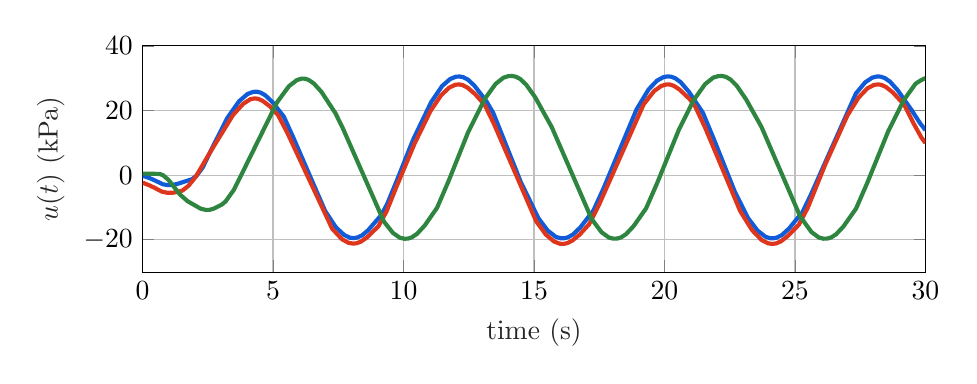
\begin{tikzpicture}

\begin{axis}[%
width=0.82\textwidth,
height=0.237\textwidth,
at={(0\textwidth,0\textwidth)},
scale only axis,
xmin=0,
xmax=30,
xlabel style={font=\color{white!15!black}},
xlabel={time (s)},
ymin=-30,
ymax=40,
ylabel style={font=\color{white!15!black}},
ylabel={$u(t)$ (kPa)},
axis background/.style={fill=white},
xmajorgrids,
ymajorgrids
]
\addplot [color=mycolor1, line width=1.5pt, forget plot]
  table[row sep=crcr]{%
0.00666666666666771	-0.179096564923768\\
0.273333333333333	-0.939244946905657\\
0.453333333333333	-1.57627562558133\\
0.780000000000001	-2.83307073668107\\
0.98	-3.10785389717242\\
1.14	-3.04568983791372\\
1.34666666666667	-2.68531847989229\\
1.9	-1.25104047496698\\
2.08	-0.111366055224206\\
2.31333333333333	2.46889286820926\\
2.64666666666667	8.06095541630684\\
3.24666666666667	17.663951179183\\
3.7	22.8578033766669\\
4.02	25.0830965124492\\
4.24	25.752486309974\\
4.38	25.8002355149119\\
4.52	25.5308579247909\\
4.7	24.7110130852921\\
4.97333333333333	22.6235619939529\\
5.41333333333333	18.0873875248582\\
5.76666666666667	11.8151240384951\\
6.99333333333334	-11.0387265588291\\
7.40666666666667	-16.131674776067\\
7.72666666666667	-18.5326489488848\\
7.95333333333333	-19.3786207118401\\
8.1	-19.4741191217158\\
8.23333333333333	-19.2939334427051\\
8.41333333333333	-18.6245436451803\\
8.64	-17.0812533044535\\
9.13333333333334	-12.4919240600505\\
9.36666666666667	-9.06028780329144\\
9.77333333333333	-1.10418914657325\\
10.3666666666667	10.9421244236882\\
11.06	22.5938313569162\\
11.48	27.5687579544021\\
11.7866666666667	29.7246796037653\\
12.0066666666667	30.4382148926477\\
12.1533333333333	30.5138928778322\\
12.2933333333333	30.275146853143\\
12.4666666666667	29.5498994951249\\
12.7133333333333	27.7111046408205\\
13.1866666666667	22.7199613322237\\
13.44	19.1982322359592\\
13.8733333333333	10.4484156631988\\
14.4933333333333	-2.11773359100853\\
15.1666666666667	-13.3036605439938\\
15.52	-17.1217950822309\\
15.8266666666667	-19.0470790624604\\
16.0133333333333	-19.5209673982586\\
16.16	-19.5218683266536\\
16.3066666666667	-19.2200573143107\\
16.5	-18.3263363464175\\
16.78	-16.1370803464373\\
17.28	-10.9044882279661\\
17.6666666666667	-4.06013521074405\\
18.9333333333333	20.388358645825\\
19.3933333333333	26.5281856581152\\
19.7133333333333	29.2255652729056\\
19.96	30.3120849173402\\
20.1266666666667	30.5472272284492\\
20.26	30.4373139642527\\
20.4133333333333	29.9634256284545\\
20.62	28.7381630111816\\
20.94	25.7371705272581\\
21.4733333333333	19.2468823692921\\
21.8866666666667	11.2295205817103\\
22.6933333333333	-5.11061771937653\\
23.2	-13.2649206230065\\
23.56	-17.1172904402556\\
23.86	-19.0254567809791\\
24.0466666666667	-19.528174825419\\
24.18	-19.5416887513448\\
24.32	-19.2876269439397\\
24.5066666666667	-18.4939090278975\\
24.7733333333333	-16.5118665587796\\
25.2866666666667	-11.4585591909241\\
25.6133333333333	-6.00343775887463\\
27.3333333333333	25.2362543396083\\
27.6866666666667	28.6723952383427\\
27.96	30.141809450675\\
28.1466666666667	30.5211003049926\\
28.28	30.4661436728944\\
28.44	30.0309952580835\\
28.64	28.912943119822\\
28.9333333333333	26.2939442754012\\
29.4666666666667	20.1315940532347\\
29.7933333333333	16.0552658635738\\
30	13.9088333645785\\
};
\addplot [color=mycolor2, line width=1.5pt, forget plot]
  table[row sep=crcr]{%
0.00666666666666771	-2.34880563633272\\
0.260000000000002	-3.15704458754234\\
0.453333333333333	-3.90067088481957\\
0.753333333333334	-5.14665485517867\\
0.953333333333333	-5.47369186258312\\
1.12666666666667	-5.47459279097817\\
1.34	-5.22503562554833\\
1.53333333333333	-4.76105750209574\\
1.76	-3.30155350210894\\
2.03333333333333	-0.578947892257013\\
2.63333333333333	7.65914135211294\\
3.46666666666667	18.6009167100387\\
3.85333333333334	22.0379585371681\\
4.13333333333333	23.4857504680192\\
4.3	23.7362085618441\\
4.42666666666667	23.5965646606108\\
4.6	22.9866361371595\\
4.87333333333333	21.31271117915\\
5.19333333333334	18.5468610063355\\
5.54	13.2214732631738\\
7.26666666666667	-16.5920491859394\\
7.64666666666667	-19.8678248303542\\
7.89333333333333	-20.9534435463938\\
8.06666666666667	-21.193090499478\\
8.2	-21.0822763068864\\
8.36666666666667	-20.5759545488663\\
8.60666666666667	-19.2218591711008\\
9.04	-15.8010340550823\\
9.35333333333334	-11.1504416798157\\
9.72	-3.78985669222798\\
10.42	9.67541910024286\\
11.0333333333333	19.8369904680522\\
11.4333333333333	24.6344341717125\\
11.7466666666667	27.0534269124314\\
11.9866666666667	27.9462469519295\\
12.1333333333333	28.0669713568667\\
12.2666666666667	27.8408383297082\\
12.4533333333333	27.0498231988512\\
12.7466666666667	25.045257519857\\
13.1133333333333	21.6902001766774\\
13.4733333333333	15.7080356335216\\
15.0866666666667	-14.3289170575648\\
15.46	-18.4290421834536\\
15.7666666666667	-20.5309081291136\\
15.9866666666667	-21.2165146377494\\
16.1333333333333	-21.2831833389834\\
16.2733333333333	-21.0462391710843\\
16.46	-20.301171388375\\
16.7533333333333	-18.3659771957999\\
17.1133333333333	-15.1793934624954\\
17.4866666666667	-9.2530864798329\\
19.2	21.8784942112436\\
19.6	25.9885295494781\\
19.8733333333333	27.5660551692169\\
20.08	28.0669713568667\\
20.2066666666667	28.0318351494596\\
20.3533333333333	27.6372285124261\\
20.5733333333333	26.4966531642883\\
20.9666666666667	23.4893541815994\\
21.18	21.1748691347068\\
21.5666666666667	14.5152064384707\\
22.9	-11.103593403273\\
23.3533333333333	-16.988457679763\\
23.72	-20.0624253636858\\
23.9733333333333	-21.1129078723183\\
24.14	-21.2894898377488\\
24.28	-21.1210162278737\\
24.4533333333333	-20.5227997735582\\
24.7133333333333	-18.9308592994985\\
25.1533333333333	-15.2947122970622\\
25.4933333333333	-10.0422997538998\\
26.16	3.28603492252286\\
27.0066666666667	18.4063161767071\\
27.4333333333333	23.953332305052\\
27.7733333333333	26.828194813668\\
28.02	27.870568966745\\
28.1866666666667	28.0759806408172\\
28.3133333333333	27.9093088877323\\
28.4866666666667	27.2516311593432\\
28.7533333333333	25.5488764926919\\
29.1866666666667	21.7550670211213\\
29.52	16.3621096483305\\
29.84	11.6834083071383\\
30	9.93014051593721\\
};
\addplot [color=mycolor3, line width=1.5pt, forget plot]
  table[row sep=crcr]{%
0.00666666666666771	0.467351734541296\\
0.413333333333334	0.433695623783223\\
0.673333333333332	0.313872147241096\\
0.793333333333333	-0.0861400601626983\\
0.993333333333332	-1.48708371447102\\
1.44666666666667	-6.08542224282451\\
1.72666666666667	-8.07647399589292\\
2.22666666666667	-10.3774451168598\\
2.42666666666667	-10.7765563958685\\
2.56666666666667	-10.734212761301\\
2.73333333333333	-10.3630302625389\\
3.03333333333333	-9.14857878600669\\
3.18	-8.15395383786753\\
3.5	-4.55294304283837\\
3.82	0.648116581805965\\
5.15333333333333	22.506441302596\\
5.60666666666667	27.4822688284769\\
5.91333333333333	29.4012463099411\\
6.10666666666667	29.8661253617887\\
6.23333333333333	29.8156733716657\\
6.37333333333333	29.4210667346322\\
6.56666666666667	28.3174294506916\\
6.85333333333334	25.7795141618256\\
7.39333333333333	19.1144458952192\\
7.66666666666667	14.6521475545188\\
9.24666666666667	-14.332520771145\\
9.59333333333333	-17.8785749340759\\
9.86	-19.3741160698648\\
10.0333333333333	-19.6903419365286\\
10.18	-19.6254750920848\\
10.32	-19.2497879513475\\
10.52	-18.1506553093821\\
10.8133333333333	-15.5812075266893\\
11.2866666666667	-10.0882471020476\\
11.72	-1.96457576384942\\
12.48	13.3521078804565\\
13.1133333333333	23.5686358803642\\
13.5266666666667	28.1940022605693\\
13.8266666666667	30.1291964531443\\
14.02	30.6247070704238\\
14.1733333333333	30.6544377074605\\
14.3066666666667	30.4373139642527\\
14.4733333333333	29.7228777469752\\
14.7	27.9786803741514\\
15.0466666666667	24.0659483544337\\
15.68	14.8548564434059\\
17.2133333333333	-13.6279947662131\\
17.5866666666667	-17.662352119263\\
17.8666666666667	-19.3011408698655\\
18.04	-19.6570075859117\\
18.1933333333333	-19.6182676649244\\
18.34	-19.2533916649277\\
18.5266666666667	-18.2749834278995\\
18.8133333333333	-15.8145479810081\\
19.2933333333333	-10.3125782724159\\
19.7133333333333	-2.58171171446113\\
20.5533333333333	14.0872654508202\\
21.1133333333333	23.1226763248126\\
21.5533333333333	28.1237298457551\\
21.8666666666667	30.1517196630207\\
22.06	30.628310784004\\
22.2133333333333	30.6517349222754\\
22.3533333333333	30.3967721864752\\
22.5333333333333	29.5616115642606\\
22.7733333333333	27.584974665513\\
23.1333333333333	23.3551158507364\\
23.72	14.8422434458752\\
25.2	-12.8009424995539\\
25.6333333333333	-17.627215911856\\
25.9133333333333	-19.3002399414704\\
26.0933333333333	-19.6651159414671\\
26.2466666666667	-19.6209704501095\\
26.3866666666667	-19.2813204451743\\
26.5733333333333	-18.3209307760472\\
26.8533333333333	-15.9379751711305\\
27.34	-10.3630302625389\\
27.7733333333333	-2.34206476137688\\
28.58	13.6998662409472\\
29.18	23.3091685025887\\
29.62	28.2642746753834\\
29.8066666666667	29.2392381861952\\
30	30.0200393252793\\
};
\end{axis}
\end{tikzpicture}%
  \caption{(top) Soft robot manipulator with three parallel embedded pneumatic bellows. This manipulator changes its posture by inflation and deflation of an embedded pneumatic network (<0.1 \si{\mega \pascal}). (bottom) Differential pressure signals applied on the internal bellows structures given by the input vector $\uB = (u_1\,u_2,\,u_3)^\top$, shown by the trajectories (\ldata{Matlab1},\ldata{Matlab2},\ldata{Matlab3}), respectively.}
  \vspace{-0.1cm}
  \label{fig:C2:soft_robot}
\end{figure}

